
\chapter{Carbon Species-Assisted Nitrogen Activation on Titania}
\section{Introduction}
This project investigates metal oxide species capable of facilitating photocatalytic nitrogen fixation. Semiconductor-based photocatalysts have long been central to photo-driven reaction studies, including water splitting, nitrogen reduction, CO$_2$ reduction, and degradation of organic pollutants \cite{INOUE1979PhotoelectrocatalyticPowders, Mao2009PromotingOrange}. Among these, metal oxides such as titanium dioxide (TiO$_2$), vanadium oxide \cite{Tennakone1993NitrogenIII}, tungsten oxide \cite{Endoh_1986, li_2016}, and carbon nitride \cite{Dong_2015, MA_2016} have been reported to enable photocatalytic nitrogen fixation. 

In 1977, Schrauzer and Guth first reported that N$_2$ can be photocatalytically reduced to NH$_3$ and N$_2$H$_4$ over TiO$_2$\cite{Schrauzer_1977}. This discovery prompted extensive investigations into semiconducting oxides and hydroxides as photocatalysts \cite{bourgeois_1988, palmisano_1988, Schrauzer_2011, Hirakawa_2017, skuldsson_2017, tennakone_1988, li_2016}. Subsequent experiments found signals of ammonia formation on titania surfaces under light exposure \cite{Bickley_1979, Augugliaro_1982, Soria_1991, Yuan_2013, Hirakawa_2017}, and further studies explored the surface chemistry of nitrogen on rutile TiO$_2$ \cite{Yates_1991, Kim2016, Kim2014, Chen_2007, Karunagaran_2007}.

Despite these experimental advances, there are relatively few computational investigations on the interaction between nitrogen and the TiO$_2$ surface. To unravel the complex nature of photocatalysis, our group performed the first in-depth computational studies of photocatalytic nitrogen fixation on titania \cite{Comer_sustainable, comer2018role}. These simulations examined the role of iron doping and anion vacancies in modulating N$_2$ activation and adsorption at active surface sites \cite{comer2018role, mao_2019, Schrauzer_1977, Hirakawa_2017, Comer_sustainable}.

Despite these advances, there are relatively few computational investigations on the interaction between nitrogen and the TiO$_2$ surface providing guidance. Our group conducted one of the first DFT studies of photocatalytic nitrogen fixation on TiO$_2$, examining the effects of Fe doping and oxygen vacancies on nitrogen adsorption and activation \cite{Comer_sustainable, comer2018role, mao_2019}. These studies highlighted that N$_2$ binds only weakly to oxygen vacancies, casting doubt on direct reduction mechanisms at these sites \cite{Huang2023FormationIllumination}.

\subsection{Competing Mechanistic Hypotheses}

Since these early efforts, growing interest has led to the emergence of three dominant mechanistic hypotheses for photocatalytic nitrogen fixation \cite{Medford_2017, Hirakawa_2017, cao2019photocatalytic, hu2016effect, zhao2019tuning, jia2019site}:

\begin{enumerate}
  \item \textbf{Direct reduction at oxygen vacancies}: This widely assumed mechanism involves electron-driven reduction of N$_2$ at or near surface oxygen vacancies on titania. However, the low overpotential ($\sim$0.1 V) at the conduction band edge of TiO$_2$ raises concerns about whether this process is kinetically feasible \cite{Hirakawa_2017, cao2019photocatalytic, hu2016effect, zhao2019tuning, jia2019site}.
  \item \textbf{Oxidative pathways on vacancies}: An alternative hypothesis suggests that photogenerated holes drive N$_2$ activation via photolysis or nitrogen oxidation, providing a much larger thermodynamic driving force. Still, weak N$_2$ binding and the absence of direct experimental evidence for NO$_x$ or hydroxyl intermediates challenge this model \cite{Comer_2018}.
  \item \textbf{Carbon species-mediated activation}: A newer hypothesis suggests that photogenerated carbon species promote N$_2$ activation. DFT calculations show strong C–N interactions (E$_{ads} \approx$ –1.89 eV) at carbon-modified TiO$_2$ surfaces \cite{comer2018role}. Supporting evidence from ambient pressure XPS and EPR experiments shows that nitrogen-containing species appear only in the presence of surface carbon \cite{comer2018role, Liu2019}.
\end{enumerate}

This third mechanism aligns with evidence from other fields. In combustion chemistry, species like \ce{CH^.} are known to activate N$_2$ via diazo intermediates \cite{glarborg2018modeling}. In homogeneous catalysis, C–N bond formation could play a role in nitrogen activation \cite{lv2020direct}. Similarly, recent electrocatalysis studies suggest that carbon species such as CO can promote the nitrogen bond cleavage \cite{chen2020coupling, huang2021direct}. These findings suggest that carbonaceous hole scavengers may serve as co-catalysts or reactants, and challenge the assumption that nitrogen is chemically inert under photocatalytic conditions involving carbonaceous species.

\subsection{Carbon-Species on TiO$_2$ Oxygen-Vacancy Site as a Model System}

\begin{figure}[h]
\centering
\includegraphics[width=\textwidth]{figures/proposal_figures/N2_redox_cycle_r3.pdf}
\caption{(a) The free energy diagram of the oxidative active site regeneration. The potential is set to that of oxidizing holes at the band edge of rutile TiO$_2$ (b) The thermodynamic cycle of N$_2$ reduction on a carbon substitution at a bridging oxygen (C*) on TiO$_2$. The path consists of a reductive portion (red) and an oxidative active site regeneration portion (blue).  (c) The free energy diagram of the reductive ammonia production portion of the thermodynamic cycle. The potential is set to that of reducing electrons at the band edge of rutile TiO$_2$. Image from Comer et al. \cite{comer2018role}.}
\label{fig:reduct_path}
\end{figure}

% Our group previously proposed a thermodynamic cycle in which a carbon substitution at a bridging oxygen site (C*) facilitates both N$_2$ binding and reduction (Figure~\ref{fig:reduct_path}) \cite{comer2018role}. This model incorporates both reduction and oxidation half-reactions, making it a compelling framework to reconcile the disparate observations in literature.




A key insight from Comer et al. was the role of carbon substitution at bridging oxygen (O-br) sites in enabling nitrogen activation on TiO$_2$ \cite{comer2018role}. Their simulations revealed strong C–N interactions and proposed a thermodynamically feasible reaction cycle at the C* site, illustrated in Figure~\ref{fig:reduct_path}. While this provides one possible pathway for photocatalytic nitrogen fixation, the identity of key surface descriptors remains uncertain. Some studies suggest that surface hydroxyls, formed via water dissociation on O-br sites, may also participate in the reaction mechanism \cite{Schaub_2001, Henderson1996, Krischok_2001, Ketteler_2007, Xie_2019}. Others also proposed that a complex balance of oxidative and reductive process could be responsible for the mechanism \cite{Comer_sustainable}.

While the C* site offers a plausible path forward, further studies are needed to clarify how carbon species influence the NRR mechanism. In this chapter, we build on the carbon species hypothesis by combining DFT simulations with experimental insights. Electron paramagnetic resonance(EPR) experiments and infrared (IR) spectroscopy conducted in the presence of methanol reveal enhanced NH$_3$ production and carbon species intermediates, suggesting a role for carbonaceous scavengers in activating nitrogen (\ref{EPR figure 1}, \ref{EPR figure 2}). Our simulations assess the thermodynamics of carbon species-mediated N$_2$ activation on TiO$_2$ and help propose a thermodynamically feasible reaction pathway consistent with these observations.

% In this chapter, we build on previous work by examining the role of carbon more closely, combining computational simulations with new experimental evidence. Recent electron paramagnetic resonance (EPR) measurements show enhanced ammonia formation when TiO$_2$ is illuminated in the presence of methanol as a carbon source. These experiments also identified surface-bound intermediates (Figures~\ref{fig:EPR}). Motivated by these findings, we present a computational study of methanol’s role in enhancing N$_2$ reduction and propose a thermodynamically viable reaction pathway informed by both theory and experiment.


\section{Overview of Theoretical Methods}
\subsection{Density Functional Theory}
In this project, we are using computational chemistry methods to study catalyst surface structure and probe reaction mechanisms at the atomic level. To simulate relevant electronic structures and calculate material energetics, we employ density functional theory (DFT). DFT is based on the first and second Hohenberg-Kohn theorems and implemented with the Kohn-Sham equations. It is a quantum mechanical atomistic simulation method to investigate the electronic structure of a many-electron system based on electron density of the system \cite{Hohenberg_1964,Kohn_1965}. The method provides significant increase in computational accuracy without additional computing time. The determination of electron density is independent of the number of electrons, because it is a physical characteristic of all molecules in the system. Therefore, DFT method does not scale exponentially as the number of electrons increases. The method only scales to the order of N$^3$ \cite{TOULHOAT_2010} (x-y-z coordinates of the individual electron), where N is the number of basis functions (typically proportional to the volume of the system). 

  
%   Exchange correlation functionals
On the other hand, a main challenge in DFT methods \cite{Burke_2012, Parr_1980} is the approximations of the electron exchange-correlation (XC) energy, since the exact form of XC energy is not known. Although TiO$_2$ has been extensively studied with computational methods \cite{Jauho_2015, Diebold_2003, Schaub_2001, Morgan_2007, Landmann_2012, De_k_2011} there is no consensus regarding the level of theory needed. In this project, we will mainly use the generalized gradient approximation (GGA) level of theory to probe the XC energy, due to its speed relative to higher level methods. In GGA, a gradient correction factor is used to probe the XC energy and account for non-uniformity of the electron density. The Bayesian error estimation functional (BEEF-vdw) \cite{beef}, a GGA with van der Waals (vdW) level of theory, will be used to describe exchange-correlation interactions and to generate an ensemble of values for the electronic energy. The ensemble allows us to quantify uncertainty on all calculated systems such that critical intermediate states with large errors can be identified. We will also use the Heyd-Scuseria-Ernzerhof functional (HSE06) \cite{hse} to more accurately probe energetics on promising metal oxide surfaces where electrons are highly delocalized \cite{Burke_2012}. HSE06 is a hybrid level theory that integrates the Fock exchange in the short-range and approximates long-range contribution by Perdew–Burke-Ernzerhof (PBE) exchange functional \cite{SAVIN_1996}. HSE06 appears to yield accurate results for semiconductors \cite{hse}, but also requires more expensive computing resources. The combination of GGA and hybrid level of theory calculations will optimize computational power distribution such that we can focus on the most relevant atomic scale systems and efficiently asses the energetics of adsorbed species on metal oxide surfaces. 
 
All stationary geometry optimizations and GGA functional calculations were performed in the Quantum ESPRESSO software package \cite{QE} together with the Atomic Simulation Package (ASE) \cite{ase}. An error estimation for each calculation can be obtained from the ensemble of values produced by BEEF-vdW \cite{Medford_2014a}. The plane-wave cutoff energy was set at 400 eV for all GGA calculations, and a Monkhorst-Pack k-point grid spacing of {$4\times4\times 1$} was used to sample the reciprocal space. The NNIN/C pseudopotentials \cite{cornell} were chosen to treat the core-electron interactions. A dipole correction was applied for all slab calculations. All geometries were optimized using the BFGS line search method to a total force of 0.05 eV/\si{\angstrom}. Gas phase calculations were performed at the $\Gamma$ point in a unit cell with 6\textup{~\AA} vacuum with all other settings identical to the slab calculations. Geometries of adsorbed surfaces were determined by trying adsorbates of multiple orientations and taking the lowest energy configuration.  

Energies of key adsorbed intermediate states determined by GGA were re-computed at the hybrid level of theory. HSE06 calculations were performed in the Simulation Package for Ab-initio Real-space Calculations (SPARC) software package \cite{SPARC}. The Monkhorst-Pack k-point grid spacing of {$4\times4\times 1$} and a mesh spacing of 0.1\textup{~\AA}, corresponding to an approximate plane-wave cutoff of 1800 ev \cite{Ecut_conversion, Abinit}, were used for calculations. For slab calculations, periodic and Dirichlet boundary conditions were prescribed in the plane and perpendicular to the plane of the slab, respectively. For gas phase molecules calculations, Dirichlet boundary conditions are employed in all three coordinate directions. The convergence tolerance on the normalized residual of electron density of the SCF iteration was set at 10\textsuperscript{-6}. The convergence tolerance on the Fock energy was set at 10\textsuperscript{-4} Hartree. The maximum number of Fock iterations was 20. The hybrid range screening parameter was set at 0.106 \cite{hse}. The parameters of all DFT simulations with both codes and exchange-correlation functionals are selected such that the numerical error is expected to be below 0.025 eV.

Since DFT implicitly calculates energies at 0 K in a perfect vacuum, we must add zero point energy (ZPE) and thermal corrections. To include ZPE and thermal contributions, vibrational frequency calculations and statistical mechanics corrections were performed using the ASE implementation. The ground state electronic energies ($E_{ele}$) calculated by DFT were converted to free energies ($G_i^o$) using the following equation:
\begin{equation}
G_i^o =E_{ele} + E_{ZPE} + \Delta H - T \Delta S
\end{equation}
where $E_{ZPE}$ is the zero point energy, $\Delta H $ and $T \Delta S$ are thermal contributions. Gas phase molecules were treated as ideal gases and adsorbates were treated with the harmonic approximation with a low-frequency cutoff of 30 $cm^{-1}$ \cite{BROGAARD_2014}.
Relative free energies were computed with respect to reference states using the formula:
\begin{equation}
G_i = G_i^o - \sum_j n_j \mu_j
\end{equation}
where  $G_i$ is the free energy of species $i$, $G_i^o $ is the total energy computed from DFT and free energy corrections, $n_i$ is the number of atoms $j$ in species $i$, and $\mu_j$ is the reference chemical potential. The reference for nitrogen was N$_2$ ($\mu_N = \frac{1}{2}G_{N_2}^o$), the reference for hydrogen was $H_2$ ($\mu_N = \frac{1}{2}G_{H_2}^o$), the reference for oxygen was $H_2O$ ($\mu_O = G_{H_2O}^o - 2\mu_H$), and the reference for carbon was $CH_3OH$ ($\mu_C = G_{CH_3OH}^o - 4\mu_H - \mu_O$). All thermodynamics were evaluated at 300 K. Gas partial pressures were set to approximate atmospheric conditions (0.8 atm N$_2$, 0.2 atm O$_2$). Liquid water was approximated as an ideal gas at saturation pressure at 300 K (0.035 atm).

\subsection{Computational Hydrogen Electrode} \label{CHE_method}
\begin{figure}[h]
\centering
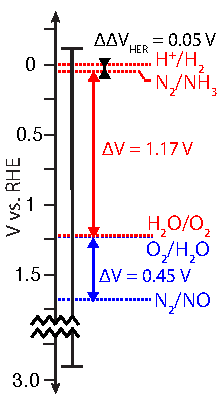
\includegraphics[width=0.2\textwidth]{figures/proposal_figures/redox_ladder.pdf}
\caption{The band edges of rutile vs common redox couples.}
\label{fig:redox_ladder}
\end{figure}

To model the thermodynamic effect of photo-excited electrons and holes, we use the computational hydrogen electrode (CHE) model. The CHE model (\ref{fig:redox_ladder}) is adopted from electrochemical studies that involve proton-electron transfer \cite{Peterson_2010, Norskov_2004,Skulason_2012} to avoid the explicit treatment of solvated protons. In this technique, the potential of the reversible hydrogen electrode (RHE) is set at zero. The free energy of reaction \ref{eq:HER} is defined to be in equilibrium at zero voltage. Hence, the chemical potential of a proton-electron pair $\mu(H^+) + \mu(e^-)$ is equal to half of the chemical potential of gaseous hydrogen $\mu(H_2)$. Therefore, the energy of each step that involves an electron transfer is varied by an energy of $eU$, where $e$ is the change in number of electrons and $U$ is the potential relative to this zero point (\ref{eq:CHE}). When utilizing the CHE model in our analysis, the major assumptions are: 1) charge transport is independent of surface kinetics; 2) electric field and solvent effects are negligible. In the current study, the relative free energies of intermediate states do not reflect any kinetic barriers since reaction barriers and coverage effects are not calculated. More accurate prediction of these kinetic information under photocatalytic conditions would require additional analysis such as an explicit potential model for charge transport and a microkinetic model for calculating relevant coverages \cite{Peterson_2010}. 
\begin{align}
	\frac{1}{2}H_2 \rightarrow H^{+}+e^{-} \label{eq:HER} \\
	\Delta G = \Delta G +eU \label{eq:CHE}
\end{align} 

\subsection{Baseline Mechanism}

\begin{figure}
\centering
\includegraphics[width=0.3\textwidth]{figures/proposal_figures/nitrogen_mechanisms.pdf}
\caption{A summary of N$_2$ fixation mechanisms. Image from van der Ham 2014\cite{van_der_Ham_2014}.}
\label{fig:N2_diss_mech}
\end{figure}

\begin{figure}[h]
\centering
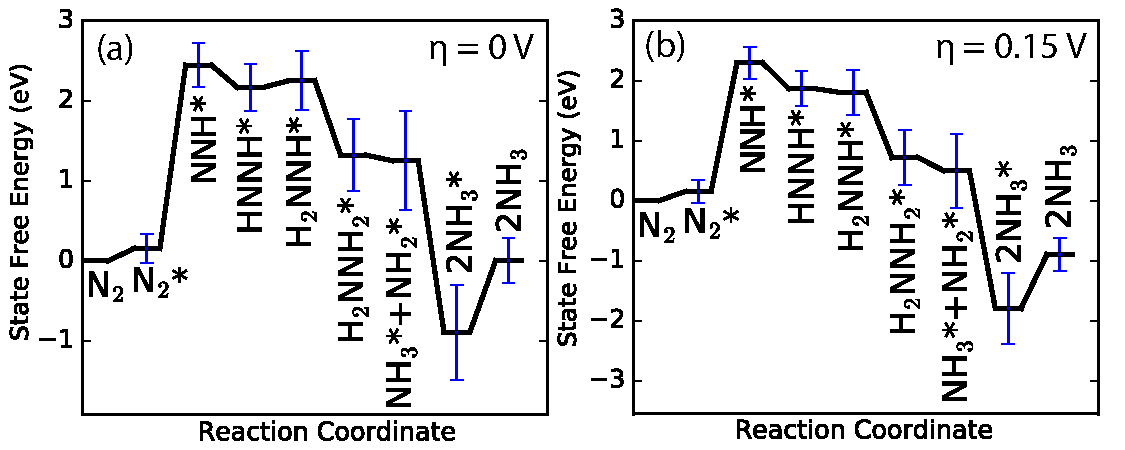
\includegraphics[width=0.7\textwidth]{figures/proposal_figures/associative_FED.pdf}
\caption{Free energy diagram for associative nitrogen reduction at an overpotential ($\eta$) of zero (a) and at the overpotential due to the conduction band edge ($\eta=0.15$ V) (b). The equilibrium potential ($\eta=0$) is computed to be 0.008 V (0.05 V experimentally). The blue error bars represent one standard deviation of the BEEF-vdW energy ensemble. Figure from Comer \cite{Comer_sustainable}.}
\label{fig:associative_FED}
\end{figure}

\begin{figure}[h]
\centering
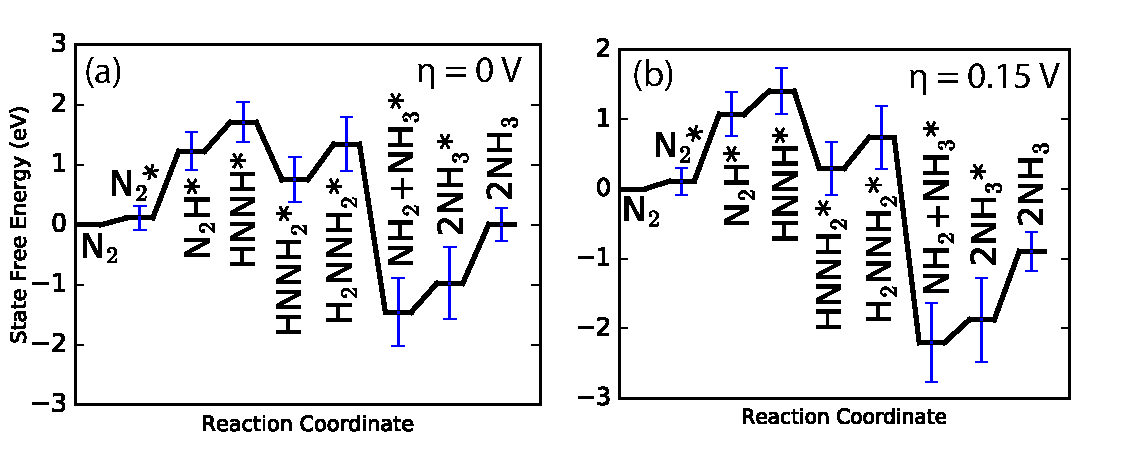
\includegraphics[width=0.7\textwidth]{figures/proposal_figures/defect_associative_FED.pdf}
\caption{Free energy diagram for associative nitrogen reduction at an O-br vacancy site at an overpotential ($\eta$) of zero (a) and at the overpotential due to the conduction band edge ($\eta=0.15$ V) (b). The equilibrium potential ($\eta=0$) is computed to be 0.008 V (0.05 V experimentally). The blue error bars represent one standard deviation of the BEEF-vdW energy ensemble. Figure from Comer \cite{Comer_sustainable}.}
\label{fig:defect_associative_FED}
\end{figure}

\ref{fig:N2_diss_mech} suggests three possible pathways for nitrogen reduction. The top pathway of \ref{fig:N2_diss_mech} is the dissociative mechanism, which requires high temperature and pressure to see reportable production rates of ammonia \cite{Honkala_2005}. Alternatively, the N-N bond can be weakened by gradual addition of hydrogen atoms to the outer nitrogen atom such that $N_2H_2$ is obtained and bond scission is enabled by desorption of ammonia, illustrated by the bottom pathway of \ref{fig:N2_diss_mech}. This is called the direct associative mechanism. We generally assume that the N-N bond breaking occurs via the associative mechanism; in this study specifically, we assume that nitrogen atoms are bonded to surface carbon and hydrogen atoms before the bond breaking occurs.
 
From previous attempts to simulate the mechanism through the direct associative mechanism, we learned that a fundamental challenge is the thermodynamic limiting potential. Previous free energy diagrams (FED) of the nitrogen reduction mechanism are shown in Figure  \ref{fig:associative_FED} and \ref{fig:defect_associative_FED}. Both diagrams show the energetics with and without reductive potentials. The NRR mechanism on pristine rutile TiO$_2$, shown in \ref{fig:associative_FED}, reveals a thermodynamic limiting potential of 2.5 eV due to the unstable NNH* adsorbed intermediate; the mechanism on the O-br site, shown in \ref{fig:defect_associative_FED}, indicates that the N$_2$H and N$_2$H$_2$ intermediates are also too unstable. To overcome this thermodynamic challenge, Comer introduced et al. CH$_4$ as the representative hydrocarbon and simulated a feasible pathway assisted by carbon species \cite{comer2018role} (\ref{fig:reduct_path}(c)). This route (\ref{fig:reduct_path}(c)) exhibits a low thermodynamic barrier of 0.55 $\pm$ 0.12 eV, which is below the threshold for a turnover frequency of 1/s for an active catalyst ($\sim$ 0.75 eV) \cite{Iriawan_2021}. From \ref{fig:reduct_path}a, the oxidation of CH$_4$* to the C* site is highly exothermic, made possible by the the strong oxidative potential of photo-generated holes on TiO$_2$ under photocatalytic conditions. In this study, we will use methanol as the representative carbon source for the following reasons. First, it acts as a more controlled carbon source and has shown to promote ammonia production in experiments. Second, as a short-chain alcohol, methanol is also thermodynamically easier to oxidize than CH$_4$ \cite{comer2018role}. Thirdly, the role of methanol has not yet been studied computationally in photocatalytic NRR.


\subsection{Finding a Thermodynamically Plausible Mechanism }
% To simulate methanol as the source of carbon species,
There are two major steps to probe in this investigation: the pathway leading to carbon-nitrogen interaction and the pathway for nitrogen fixation, both of which occur on the TiO$_2$ active site. To find reasonable pathways for these two steps, we first found the energies of all intermediate states along the path. Then, infeasible intermediate states were ruled out if the formation energy was exceedingly high (more than 1 eV) or the intermediate was not adsorbed on the surface with a stable geometry. 

% Since a carbon-assisted nitrogen fixation pathway was already suggested in \ref{fig:reduct_path}(c),
For the carbon specie formation pathway, methanol was used as a representative carbon source. In this pathway, the relevant intermediates are CH$_x$OH, CH$_x$OHN$_2$, CH$_x$N$_2$ and CH$_x$, with x between 0 and 3. For the direct associative nitrogen reduction pathway, relevant species are CH$_x$N$_y$H$_z$, with x  between 0 and 3, y between 1 and 2, and z between 0 to 6. We assumed that the first state is CH$_x$N$_2$ since CH was reported to be sufficiently reactive to attack the strong N$_2$ bond \cite{Glarborg_2018}.

Next, free energies calculations were performed on all relevant species to produce candidate pathways. A FED was generated for each proposed pathway. Any pathway with intermediate state that requires a high positive thermodynamic energy would be ruled out. The path was refined iteratively until a low energy pathway is found.

\section{Results}

\subsection{Carbon-Assisted Nitrogen Fixation Pathways}

\begin{figure}
    \centering
    \includegraphics[width=\linewidth]{figures/proposal_figures/Fig3_10_23_23.jpg}
    \caption{(a) Free energy diagram of photocatalytic nitrogen fixation on titania with the existence of methanol. (b) Free energy diagram of photocatalytic nitrogen fixation on titania without methanol. The thermodynamic barrier is calculated as the largest energy barrier along the reduction pathway. Thermodynamic barriers for different mechanisms: 0.55 eV (from step 9 to step 11 for the carbon-assisted mechanism); 1.48 eV (from step 0 to step 3 for the oxygen vacancy mechanism); 2.01 eV (from step 0 to step 3 for the OH-assisted mechanism). Note that oxidative steps are not included in this calculation, as they have a large driving force due to the strong oxidizing potential of photogenerated holes on titania, and the desorption of NH$_3$ is also excluded, assuming it is in equilibrium with desorbed NH$_3$.}
    \label{fig:BEEF_full_fig}
\end{figure}

\begin{figure}[h]
    \centering
    \begin{subfigure}[t]{0.44\textwidth}
        \centering
        \includegraphics[width=\textwidth]{figures/proposal_figures/CH_RHE.png}
        \caption{}
        % \caption{Free energy diagram under applied potentials}
        \label{fig:CH_RHE_a}
    \end{subfigure}
    \hfill
    \begin{subfigure}[t]{0.44\textwidth}
        \centering
        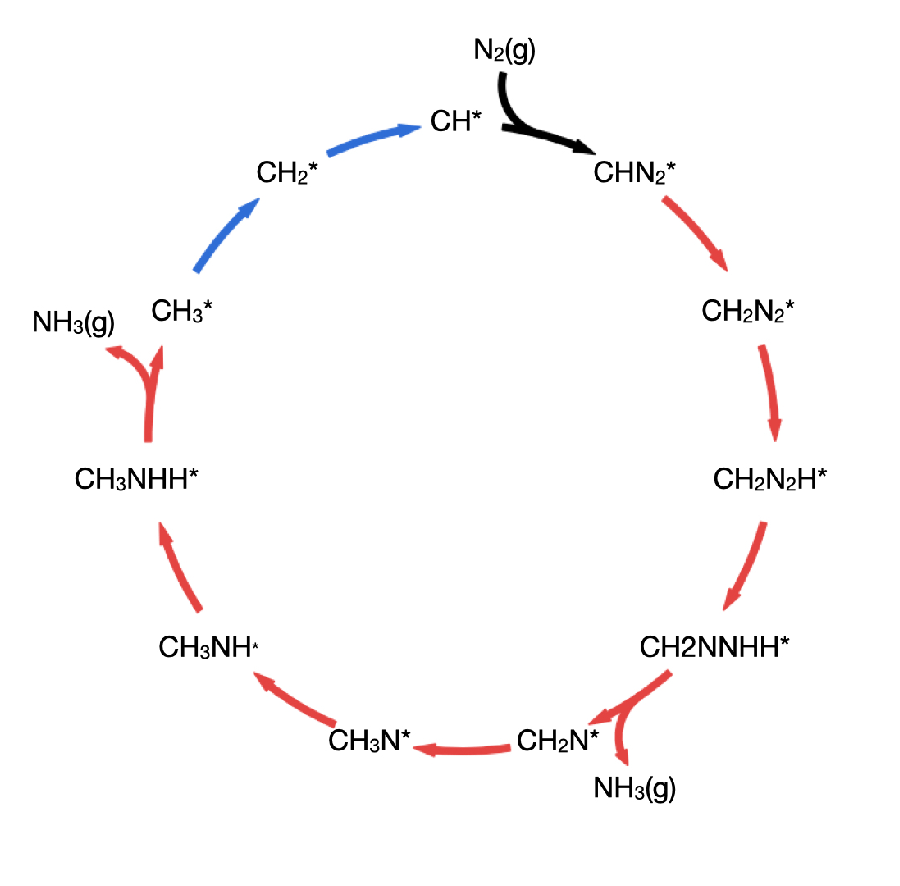
\includegraphics[width=\textwidth]{figures/proposal_figures/catalytic_cycle.pdf}
        \caption{}
        % \caption{Closed catalytic cycle for carbon-assisted nitrogen fixation}
        \label{fig:CH_RHE_b}
    \end{subfigure}
    \caption{(a) Proposed free energy diagram for nitrogen fixation with applied reductive and oxidative potential. (b) Complete catalytic cycle, with oxidation steps shown in blue and reduction steps in red.}
    \label{fig:CH_RHE_combined}
\end{figure}

% We proposed several thermodynamically feasible mechanisms for carbon-assisted nitrogen fixation starting from methanol-derived carbon radicals (CH*, CH$_2$*, CH$_3$*). These pathways converge on a common intermediate, CH$_2$N$_2$*, which then proceeds through hydrogenation steps to form ammonia (\ref{fig:BEEF_full_fig}(a)). Steps 0–11 correspond to N$_2$ fixation, while steps 12–14 represent regeneration of the carbon-based active site. The highest thermodynamic barrier in the ammonia formation portion of the cycle is under 1 eV (without applied potentials), although the regeneration steps require significant driving force. When applying a redox potential using the CHE model, regeneration becomes thermodynamically favorable due to the highly oxidative valence band edge of TiO$_2$ (2.9 V vs. RHE), as shown in ~\ref{fig:CH_RHE_a}.

We proposed several thermodynamically feasible mechanisms for carbon-assisted nitrogen fixation. Starting from methanol-derived carbon radicals (CH*, CH$_2$*, CH$_3$*), these pathways (\ref{fig:BEEF_full_fig} (a) merge on the CH$_2$N$_2$* intermediate state, which then proceeds through hydrogenation steps to form ammonia. Then the nitrogen fixation pathway can terminate in NH$_3$ formation in step 11. To close the catalytic cycle, active sites are regenerated via photo-oxidation of the surface carbon radicals in step 12 to 14. From \ref{fig:BEEF_full_fig} (a), we observe that the highest thermodynamic barrier for the formation of ammonia (steps 0-11) mechanism is less than 1 eV, when no redox potential is applied, although the regeneration of active sites requires significant driving force (steps 11-13). When applying a redox potential using the CHE model, regeneration becomes thermodynamically favorable due to the highly oxidative valence band edge of TiO$_2$ (2.9 V vs. RHE), as shown in ~\ref{fig:CH_RHE_a}, enabling the regeneration of active site and completion of this catalytic cycle (\ref{fig:CH_RHE_b}).

\subsection{Experimental Support from Spectroscopy}
\begin{figure}
    \centering
    \includegraphics[width=1\linewidth]{figures/proposal_figures/Fig1_6_14_23.jpg}
    \caption{(a) EPR spectra of titania with 5 vol\% methanol solution at 4.2 K under argon environment with and without illumination. (b)  EPR spectra of titania with 5 vol\% methanol solution at 4.2 K under nitrogen environment with and without illumination. (c) EPR spectra of titania without methanol at 4.2 K under argon environment with and without illumination. (d) EPR spectra of titania without methanol at 4.2 K under nitrogen environment with and without illumination.}
    \label{EPR figure 1}
\end{figure}


\begin{figure}
    \centering
    \includegraphics[width=\linewidth]{figures/proposal_figures/Fig2_6_11_23.jpg}
    \caption{IR spectra of titania with 5 vol\% methanol solution (a) under argon environment and (b) nitrogen environment during illumination. Trends of intensities with time of targeted wave-numbers under (c) argon environment and (d) nitrogen environment during illumination.}
    \label{EPR figure 2}
\end{figure}

\begin{figure}[h]
\centering
\includegraphics[width=0.3\textwidth]{figures/proposal_figures/step_3.png}
\caption{Step 3 to 4 of \ref{fig:BEEF_full_fig} visualized.}
\label{fig:step_3}
\end{figure}
The proposed intermediates and mechanisms are consistent with observations from EPR spectra (\ref{EPR figure 1}). Specifically, the disappearance of the CH$_2$OH* signal in N$_2$ environment and the emergence of CH$_x$N$_2$ radical signals support the formation of CH$_2$N$_2$* intermediates (\ref{fig:step_3}). When N$_2$ is present in the environment, the CH$_2$ group dissociates from the surface CH$_2$OH and binds with N$_2$, forming CH$_2$N$_2$* that is strongly adsorbed on the surface, leaving the OH* group on the active site. The uphill barrier from step 5 to 6 suggests that CH$_2$N$_2$H* and CH$_2$NNHH* may accumulate and contribute to the CH$_x$N$_2$ signal. Since CHx structures are formed in a metastable process, the systems needs sufficient surface coverage of CH$_3$NH* to overcome the energy barrier. Thus the CH$_2$N$_2$H* and CH$_2$NNHH* species are hypothesized to be responsible for the CHxN$_2$ signal in the EPR spectra.

To further confirm carbon–nitrogen interactions, in situ IR spectroscopy revealed the appearance of a C–N stretching band (1018 cm$^{-1}$) only in nitrogen environments when methanol was present and under illumination (\ref{EPR figure 2}). Control experiments without methanol or under Ar showed no such feature. These observations agree with the DFT-predicted CH$_2$N$_2$ formation pathway and indicate photo-driven carbon-nitrogen interaction on TiO$_2$.

\subsection{Validation with Hybrid Functionals}

\begin{figure}[h]
\centering
\includegraphics[width=0.5\textwidth]{figures/proposal_figures/HSE_full_fig.png}
\caption{Free energy diagram of all nitrogen fixation pathways at the oxygen-vacancy site. Zero is set to the energy of the oxygen-vacancy site. $CH$ and $CH_3$ pathways energies were adjusted to ensure alignment with the methanol pathway calculated by HSE06 functional.}
\label{fig:HSE_full_fig}
\end{figure}

Hybrid functionals such as HSE06 have demonstrated improved accuracy in describing electronic properties of titanium oxides, particularly in capturing band gaps and defect energetics \cite{hse}. To assess the robustness of our proposed mechanism, we compared free energy diagrams computed using the generalized gradient approximation (BEEF-vdW) and the hybrid HSE06 functional (\ref{fig:HSE_full_fig}). Structures were first optimized and vibrational frequencies evaluated using BEEF-vdW \cite{beef}, then single point energy calculations were performed with HSE06.

While there are quantitative differences, especially in the formation energy of ammonia, which BEEF-vdW tends to overestimate and HSE tends to underestimate, both methods yield qualitatively consistent results. In particular, both functionals support the thermodynamic viability of the carbon-assisted nitrogen fixation pathway on TiO$_2$. Although hybrid functionals offer improved treatment of electronic structure, the discrepancy in NH$_3$ formation energies suggests that neither functional is superior for all intermediates in this reaction network. Nevertheless, the qualitative agreement provides confidence in the mechanism.

These results show that carbon-based active sites offer a thermodynamically feasible route for photocatalytic nitrogen fixation on TiO$_2$. While methanol can initiate carbon radical formation, the catalytic cycle can sustain itself through surface-mediated regeneration, suggesting methanol is not strictly required once surface carbon species are present.


\subsection{Mechanistic Comparison}

We also assessed the energetics of methanol-free systems (\ref{fig:BEEF_full_fig} (b)). In the absence of carbon, both the oxygen vacancy mechanism and the hydroxyl-assisted pathway exhibit high energy barriers (1.48 and 2.01 eV, respectively) \cite{xie2019probing}, compared to $\leq$ 0.55 eV in the carbon-assisted case. These results explain why no nitrogen-centered radicals were observed by EPR in methanol-free systems (\ref{EPR figure 1} d), and demonstrate that the presence of carbon sources offers a more thermodynamically feasible route for the photocatalytic nitrogen fixation reaction through reactions with carbon intermediates.

\section{Conclusion}
Here, we used various spectroscopic techniques to investigate the interaction between carbon radicals and dinitrogen on illuminated titania. DFT simulations along with EPR and in sity IR measurements support a reaction mechanism in which CH$_2$OH* or CH* species formed via methanol oxidation or hydrocarbon contamination couple with N$_2$ to form CH$_2$N$_2$, followed by hydrogenation to methylamine and ammonia. Although this process requires 8+ electron transfers and suffers from strong NH$_3$ binding (limiting its solution-phase concentration), the spectroscopic evidence and computed energetics make this the most plausible molecular-scale mechanism photocatalytic nitrogen fixation on TiO$_2$. Future work should quantify reaction rates and efficiencies via isotopic labeling and expand mechanistic modeling to include excited-state and kinetic effects.



% We conducted electron paramagnetic resonance (EPR) measurements to observe the formation of radicals (e.g. diazo- and nitrogen-centered radicals) during photocatalytic pr/ocesses and to identify intermediates during the interaction of radicals with nitrogen. We then used in situ infrared (IR) spectroscopy to identify functional groups on the catalyst surface during the photocatalytic reaction. Finally, DFT simulations were employed to evaluate the ground-state free energies of intermediate states to identify thermodynamic barriers and the most stable molecular structures with and without carbon. The results reveal consistent evidence that carbon radicals interact with dinitrogen on illuminated titania surfaces.


